% Ce fichier main.tex est le fichier principal \`{a} partir duquel tout est g\'{e}n\'{e}r\'{e}
% This file is the main file where the final document is generated
\documentclass{these-dbl}

% Fill the pdf metadata
\hypersetup{
%    pdfauthor   = {XYZ},
%    pdftitle    = {Th\`{e}se de doctorat de XYZ},
%    pdfsubject  = {Th\`{e}se de doctorat de XYZ},
%    pdfkeywords = {mots-cl\'{e}s},
}

\geometry{vmargin=4.0cm}
\addbibresource{./biblio/biblio.bib}

\makeglossaries
% Acronymes
\newacronym{dof}{DOF}{Degree Of Freedom}
\newacronym{gui}{GUI}{Graphical User Interface}
% \newacronym{fc}{FC}{Flight Controller}
\newacronym{gcs}{GCS}{Ground Control Station}
\newacronym{ros}{ROS}{Robot Operating System}
\newacronym{ros2}{ROS2}{Robot Operating System 2}
\newacronym{sitl}{SITL}{Software-In-The-Loop}
\newacronym{lidar}{LiDAR}{Light Detection And Ranging}
\newacronym{qos}{QOS}{Quality Of Services}
\newacronym{mavlink}{MAVLink}{Micro Air Vehicle Link}
\newacronym{rtos}{RTOS}{Real-Time Operating System}


% Définitions
% \newglossaryentry{MAVLink}
% {
%     name={MAVLink},
%     description={
%         MAVLink is a very lightweight messaging protocol for communicating with drones (and between onboard drone components).
%     }
% }
  

\begin{document}

% La page de garde est en français
% The front cover is in French
\selectlanguage{french}

% S8 or S10
\semester{Semestre 8}
\entreprise{Upteko ApS}
\author{Paul WALCZAK}
\title{« Titre du stage»}
\date{« date»}
\dates{du 06 Mars 2023 au 04 Aôut 2023}
\lieu{« Lieu »}
\mail{p9walcza@enib.fr}

\jury{
{\normalTwelve \textbf{Composition du Jury :}}\\
\newline
\footnotesizeTwelve
\begin{tabular}{@{}lll}
Tuteur ENIB :          & Alexis MICHEL  & Directeur de l'ENIB\\
Accesseur :          & Pr\'{e}nom NOM & ENIB \\
Tuteur Entreprise :    & Vincent KLYVERTS TOFTERUP & Responsable du développement des drones \\
\end{tabular}
}

\maketitle



\selectlanguage{english}

\clearemptydoublepage
\chapter*{Acknowledgement}

I would like to express my deepest appreciation to all those who provided me the possibility to complete this report. A special gratitude I give to my internship supervisor, whose contribution in stimulating suggestions and encouragement, helped me to coordinate my project especially in writing this report.
\\ \\
Furthermore, I would also like to acknowledge with much appreciation the crucial role of the staff at Upteko, who gave the permission to use all required equipment and the necessary materials to complete the task. A special thanks goes to my colleagues who helped me in many ways and were always willing to help when I ran into trouble.
\\ \\
I would also like to thank my school for providing me with this wonderful opportunity to apply my academic knowledge in a real-world scenario. The experience has been invaluable and I am grateful for the skills I have acquired and the insights I have gained.
\\ \\
Finally, I express my warm thanks to my family and friends for their understanding, endless patience and encouragement when it was most required. Their moral support has made this journey easier.


\frontmatter
\clearemptydoublepage
\renewcommand{\contentsname}{Table Of Content}
\tableofcontents %sommaire %table of content
%\shorttableofcontents{Sommaire}{0}

\clearemptydoublepage
\listoffigures

\clearemptydoublepage
\listoftables

%%\clearemptydoublepage
%%\lstlistoflistings

\clearemptydoublepage
\chapter*{Introduction}
\addcontentsline{toc}{chapter}{Introduction}
\chaptermark{Introduction}

This report provides a detailed account of my internship experience at Upteko, a company that is experiencing rapid growth and is characterized by its diverse and dynamic work environment. Upteko operates in a multitude of fields, including but not limited to hardware, software, simulation, fundraising, and professional events. This diversity offers a unique learning experience, presenting an opportunity to gain exposure to a wide range of disciplines and technologies. It also poses its own set of challenges, as the breadth of the company's operations can sometimes be challeging for trainees.
\\ \\
The report begins with a comprehensive presentation of the company, outlining its field of activity, history, legal and social model, economic model, and type of work organization. This is followed by a detailed description of the projects I was involved in during my internship, including the \texttt{STM32 IMU project}, the \texttt{LogViewer project}, and the \texttt{Collision Avoidance SITL project}. Each project section provides an overview of the tasks I undertook, the challenges I encountered, and the solutions I developed.
\\ \\
Throughout the report, I aim to highlight the knowledge and skills I acquired during my internship, as well as the insights I gained into the complexities and peculiarities of working in such a multifaceted environment. The report also includes a list of codes used in the projects, providing a technical perspective on the work carried out.

\clearemptydoublepage
\chapter{Company presentation}

\section{Field of activity}
\subsection{Wind energy}
Upteko has been manually inspecting wind-turbines since 2018. Today, they are using this data and knowledge to build a system to automatically inspect wind turbines
Upteko's autonomous drone system will provide high-quality aerial data for all inspections and maintenance requirements, in a safer, more efficient manner, without causing operational downtime.
Their drones are pre-programmed with geo-referenced 3D trajectories for the inspection of wind turbines. While flying the planned routes, several images are acquired. The actual number depends on the camera specification, flight altitude and post-processing performance (overlap between images). All images are georeferenced using the UAV position at the acquisition time and these images are afterwards stitched together and in one picture on which the locations of the damages are shown.
They deliver these data as per the clients' requirements in raw files or provide a damage report that explains the severity of damages from type 1 to type 5.

\subsection{Oil and Gas}
Upteko is working on a solution for detecting oil spills on the surface of the water. They are developing payloads for their drone system that can help detect the signature of oil floating on water surfaces. This payload can be installed on Lärke and can be used to automatically or manually detect oil spills.
Upteko have developed an application to detect pirate attacks on off-shore oil rigs and large commercial ships. Pirates use small ships to attack these oil rigs and large commercial ships at night. They take the crew and contents hostage. There are no mobile long-range detection tools with aerial insight to give the crew information about nearby pirates. This results not only in huge loss to the oil industry but also endangers the crew at huge life risks.
The total cost of piracy to the shipping industry, from insurance and time lost, is estimated at over €6B/year.
Upteko's multipurpose drone system has a feature called perimeter control. This feature allows any member of the crew to investigate surrounding vessels approaching the premises. A built-in feature within the drone system is added to allow a crew member to operate and control the aerial camera in any direction with no prior drone experience. The geothermic cameras and the infrared sensors help to detect the approach of any pirates faster even during night-time.

\subsection{Offshore and Maritime}
Upteko has been consistently involved with the maritime industry since its inception. They are developing a drone system solution to live on the ship, to connect port operations on the ground and at the sea, with insight from the sky. This system includes a drone and a charging station for the drone that will be installed on the ship. The drone can autonomously perform a variety of tasks and then fly back and charge its batteries while staying protected against the weather. 
With an in-depth understanding of the challenges that the maritime industries face in attempting long and expensive inspections and other operational tasks, Upteko's software and hardware drone system allows a 100\% automatic inspection of a ship in less than 2 hours. 
Having a permanent drone on a ship will be extremely helpful in a number of cases that can range from Search and Rescue (SAR) operations, vessel docking, dry dock inspections, fire hazard detection and situational awareness among other functionalities.

\section{History}
Upteko™ was founded in 2018 by Mads Joergensen, Benjamin Mejnertz, and Sebastian Duus to pursue the opportunity of developing drone applications for the maritime sector. For Benjamin and Sebastian, it started as a hobby, competing in RC Helicopter competitions around the world and later became a business worth pursuing. Mads came onboard, and together they created Upteko and built a great team of experienced drone pilots, software- and hardware engineers, and business developers. Today Upteko has offices located in Copenhagen, Odense, and Skanderborg. Upteko is about using their creativity and initiative to become leaders in the drone industry.
To develop fitting solutions to your needs, they value collaboration and co-creation highly among external parties. Through several years of collaborating with their customers, complementary assets providers, and even competitors, they have achieved priceless partnership within the maritime and other sectors. They are continuously on the hunt for new collaborations.

\section{Legal and social model}
In Denmark, most companies operate under a legal structure of a private limited company (Anpartsselskab, ApS) as Upteko. The country has strong social welfare systems and labor laws, which mandate fair treatment and protection of employees. Danish companies usually have a strong focus on maintaining a healthy work-life balance and uphold high ethical standards, both socially and environmentally.

\section{Economic model}
Denmark follows a mixed-market capitalist system, combining free market principles with a strong regulatory oversight. Upteko operates under a model of sustainable growth, focusing on long-term stability rather than short-term profits. This includes social responsibility, ethical business practices, and environmental sustainability.

\section{Type of work organization}
Denmark has a distinctive workplace culture, often characterized by a flat organizational structure. This implies low power distance, high levels of trust, and extensive collaboration between different levels of the organization. Danish companies typically have strong communication and decision-making practices, promoting employee empowerment and autonomy.

\clearemptydoublepage
\chapter{Projects}

\section{STM32 IMU}
\subsection{PModNav}
The purpose is to get the \texttt{roll}, \texttt{pitch} and \texttt{yaw} from the PModNav to plot a 3D visualization of the IMU. The final purpose of it is to create log files from the orientation and attitude of the drone in real-time. By combining data from accelerometers, gyroscopes and magnetometers, an IMU can provide information about the object's position, orientation and angular velocity. This is crucial for tasks such as safety deployement or drone tracking.
The STM32-L4796ZG recovers the value of the sensors from the \texttt{PModNav} via \texttt{SPI Bus} and transmits them to the HMI via \texttt{UART} connection.
\begin{figure}[H]
    \centering
    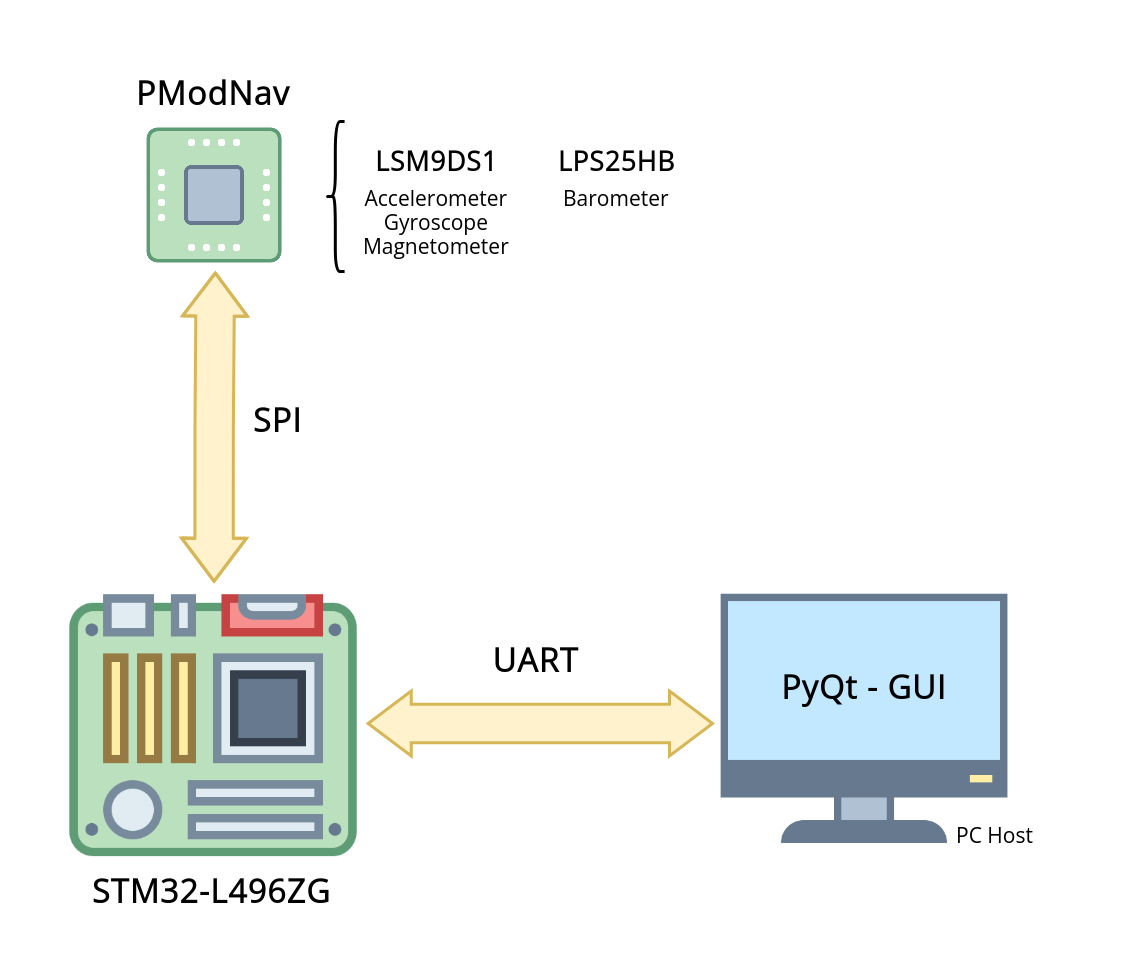
\includegraphics[width=0.65\linewidth]{./projects/pmodnav/com.png}
    \caption{Project communication overview}
\end{figure}

\subsubsection{Hardware}
The PModNav module is equipped with the \texttt{LSM9DS1}\cite{LSM9DS1_digilent_lib} sensor, offering 10-degrees-of-freedom (10-DOF) functionality. It integrates a 3-axis accelerometer, 3-axis gyroscope, 3-axis magnetometer, and an LPS25HB digital barometer. This comprehensive sensor suite allows users to obtain orientation-related data and determine the precise position and heading of the module. The module supports various full-scale options for linear acceleration, angular rate, and magnetic field measurements. It follows the Digilent Interface Specification Type 2A and utilizes a 12-pin Pmod connector with an SPI interface.

\subsubsection{Software and Development Environment}
The development environment for the PModNav project is STM32 CubeIDE. The documentation references project sources, including code snippets and libraries, such as the PModNav driver and Madgwick's filter implementation. 

\subsubsection{Data Processing}
The project outlines two approaches for deriving object attitudes: Euler angles and quaternions. Euler angles are obtained through the integration of angular velocity and provide information about the roll, pitch, and yaw of an object. However, a challenge known as \texttt{Gimbal Lock}\cite{gimbal_lock} arises when using Euler angles directly, resulting in a loss of a degree of freedom when two axes of rotation overlap. To overcome this, quaternions are introduced as a mathematical representation of displacement and rotation. They effectively resolve the Gimbal Lock issue and provide a more robust solution for determining attitudes.
\begin{figure}[H]
    \centering
    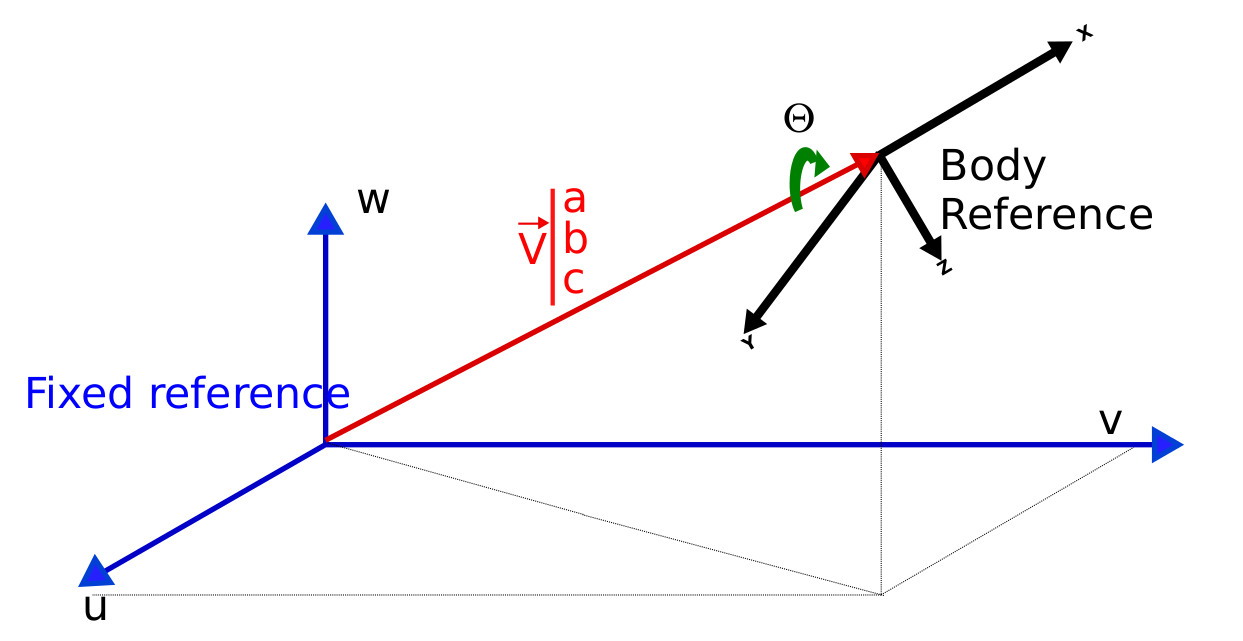
\includegraphics[width=0.65\linewidth]{./projects/pmodnav/quaternions.png}
    \caption{Quaternion representation}
\end{figure}
$$ Q = [q_0, q_1, q_2, q_3 ] $$
$$ Q = \big[cos(\frac{\theta}{2}), a.sin(\frac{\theta}{2}), b.sin(\frac{\theta}{2}), c.sin(\frac{\theta}{2})\big] $$
At each \texttt{Te}, we can calculate the new value of the quaternion vector from the velocity :
$$ Q_{k+1} = Q_k+\frac{1}{2}.T_e.\omega_k.Q_k $$
For cheap IMUs, it is unavoidable to perform a data fusion to make the accelerometer compensate for the gyroscope defect. If using a Kalmann filter is possible, there are other (faster) algorithms like Madgwick's. The idea is to compensate for the gyroscope measurement error by modulating its values by the result of a comparison between an estimate of the gravity field and the measured gravity field (with the accelerometer).
\begin{figure}[H]
    \centering
    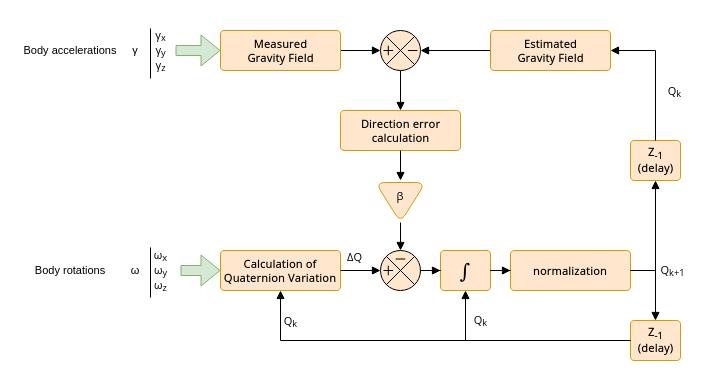
\includegraphics[width=0.9\linewidth]{./projects/pmodnav/madgwick.png}
    \caption{Madgwick filter schematic}
\end{figure}
I decided to use the most popular open source algorithm to compute rotations, the \texttt{Madgwick's algorithm}\cite{Madgwick}. This calculation updates the quaternion, from which the attitudes (Euler angles) can be calculated.
\begin{figure}[H]
    \centering
    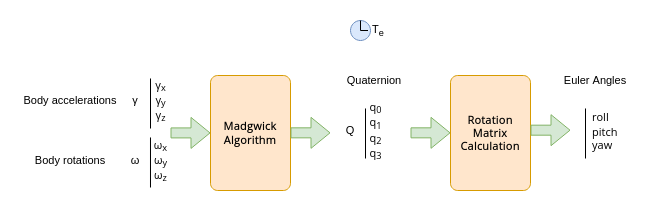
\includegraphics[width=0.9\linewidth]{./projects/pmodnav/madgwick_applied.png}
    \caption{Data transform schematic}
\end{figure}
$$ R_{12} = 2.(q_1.q_2+q_0.q_3) $$
$$ R_{22} = q_0^2+q_1^2-q_2^2-q_3^2 $$
$$ R_{31} = 2.(q_0.q_1+q_2.q_3) $$
$$ R_{32} = 2.(q_1.q_3-q_0.q_2) $$
$$ R_{33} = q_0^2-q_1^2-q_2^2+q_3^2 $$
Calculation of the Euler Angles from the rotation matrix :
$$ roll = atan2(R_{31},R_{33}) $$
$$ pitch = asin(R_{32}) $$
$$ yaw = atan2(R_{12},R_{22}) $$


\subsection{Graphical User Interface}
Additionally, a graphical user interface (GUI) is provided, leveraging \texttt{PyQt5}\cite{pyqt5} and \texttt{PyOpenGL}\cite{pyopengl} modules. The GUI manages the main window and handles OpenGL object management. It offers features like port selection and serial communication. The received data is displayed in a textbox within the GUI, facilitating real-time monitoring and analysis.
Here is how the GUI is threaded :
\begin{figure}[H]
    \centering
    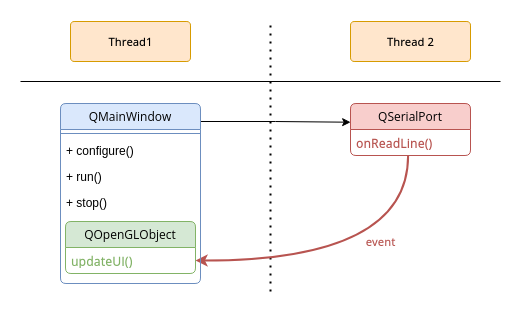
\includegraphics[width=0.65\linewidth]{./projects/pmodnav/gui_threads.png}
    \caption{Python GUI threads schematic}
\end{figure}
The use is rather simple for the communication configuration (\colorbox{cyan}{cyan box}) :
\begin{itemize}
    \item the port
    \item the baud rate
    \item the number of bits per frame
    \item the number of stop bits
    \item the parity
    \item the flow control
\end{itemize}
\begin{figure}[H]
    \centering
    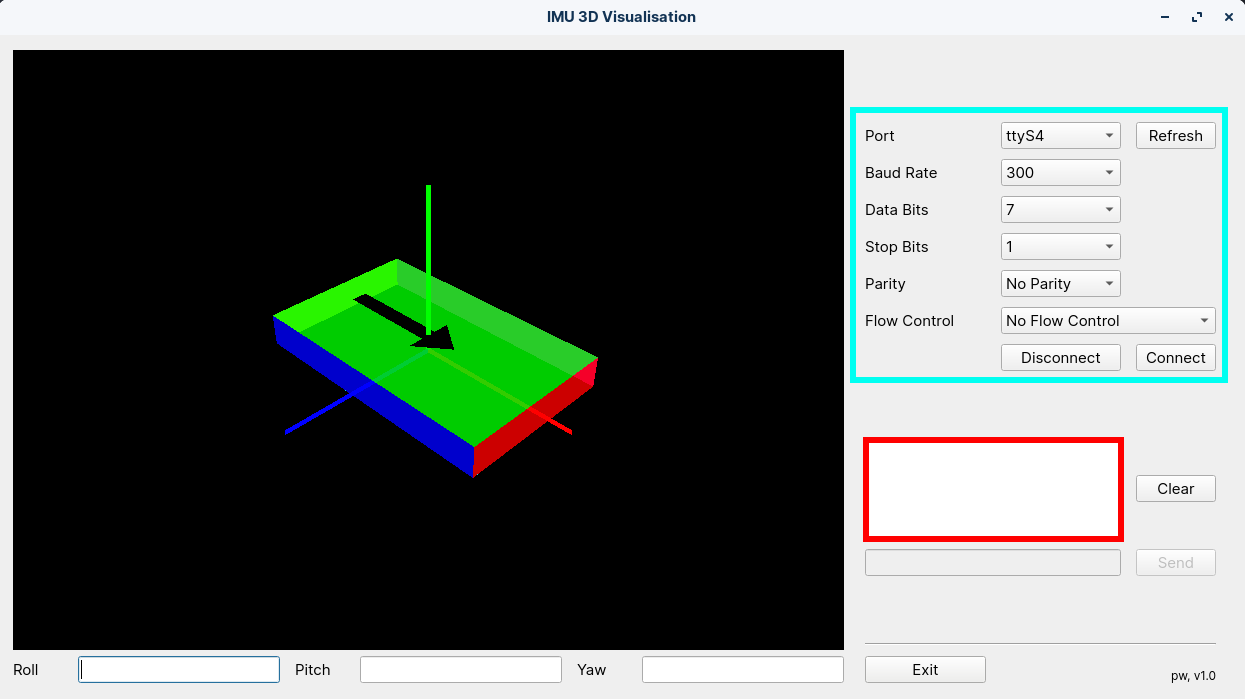
\includegraphics[width=0.65\linewidth]{./projects/pmodnav/gui_window.png}
    \caption{Python GUI window screenshot}
\end{figure}
Then click on \texttt{Connect} to start the serial communication. Every received line appeared in the textBox (\colorbox{red}{red box}).

\subsubsection{Final result}
% \begin{figure}[H]
%     \centering
%     \includegraphics{./projects/pmodnav/pmodnav_gui_record.gif}
%     \caption{Python GUI window GIF}
% \end{figure}

\subsection{Telemetry data}


\section{LogViewer}
The objective of a log viewer application is to facilitate the efficient viewing and analysis of log data generated by systems or applications. This scientific report highlights the key goals and functionality of a log viewer, which includes log visualization, search and filtering capabilities, log analysis and insights, integration with other tools, and customization options.
\subsection{Sensors tests}

\begin{figure}[H]
    \centering
    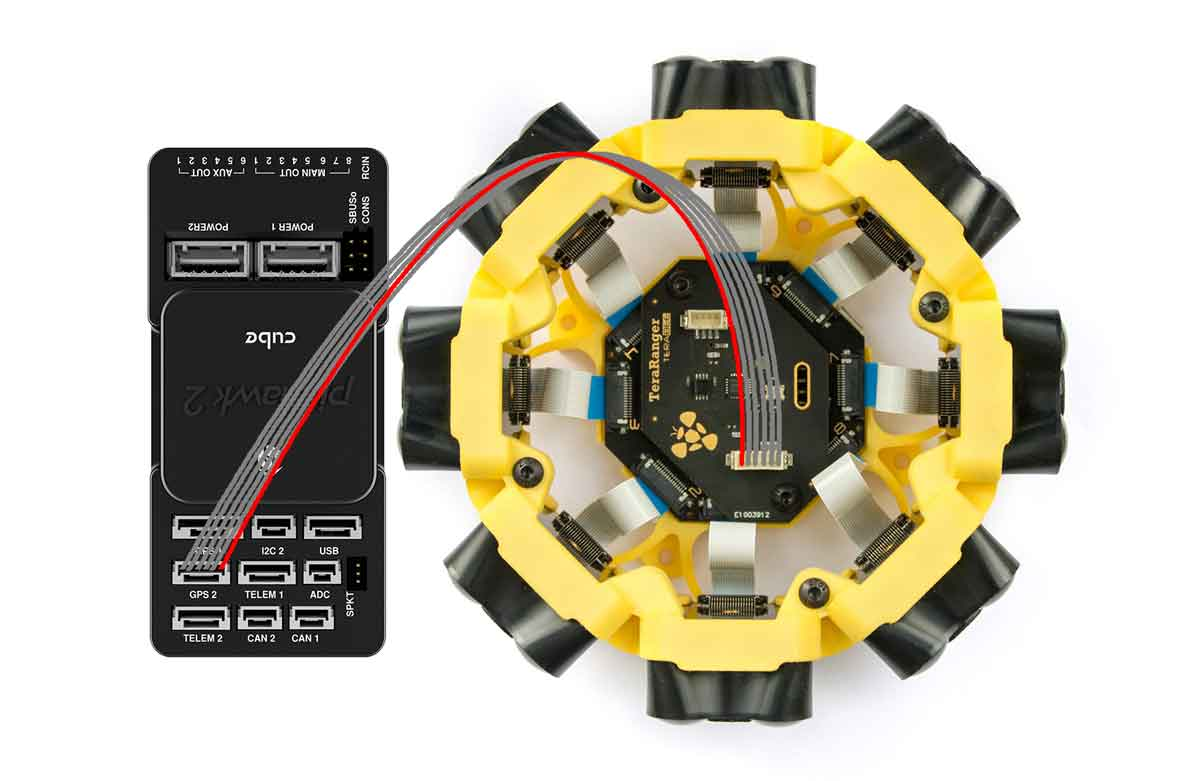
\includegraphics[width=0.65\linewidth]{./projects/logviewer/tower_evo_pixhawk.jpg}
    \caption{Terabee TowerEvo sensors and Pixhawk FlightController}
\end{figure}


\begin{table}[H]
    \centering
    \begin{tabular}{|l||l|l|}
    \hline
                      & TowerEvo & Description                 \\
    \hline
    PRX\_ORIENT       & 0        & Default                     \\
    PRX\_TYPE         & 6        & TeraRangerTowerEvo          \\
    SERIAL\_BAUD      & 921600   & serial baud                 \\
    SERIAL\_PROTOCOLE & 11       & Lidar 360 deg               \\
    AVOID\_ANGLE      & 1300     & max  lean angle             \\
    AVOID\_BEHAVE     & 1        & Stop when obstacle detected \\
    AVOID\_DIST\_MAX  & 5        & max distance avoidance      \\
    AVOID\_ENABLE     & 3        & Enable drone reaction       \\
    AVOID\_MARGIN     & 3        & min distance avoidance      \\
    \hline
    \end{tabular}
    \caption{Ardupilot flight controller configuration}
    \label{table:fc_config}
\end{table}

\begin{figure}[H]
    \centering
    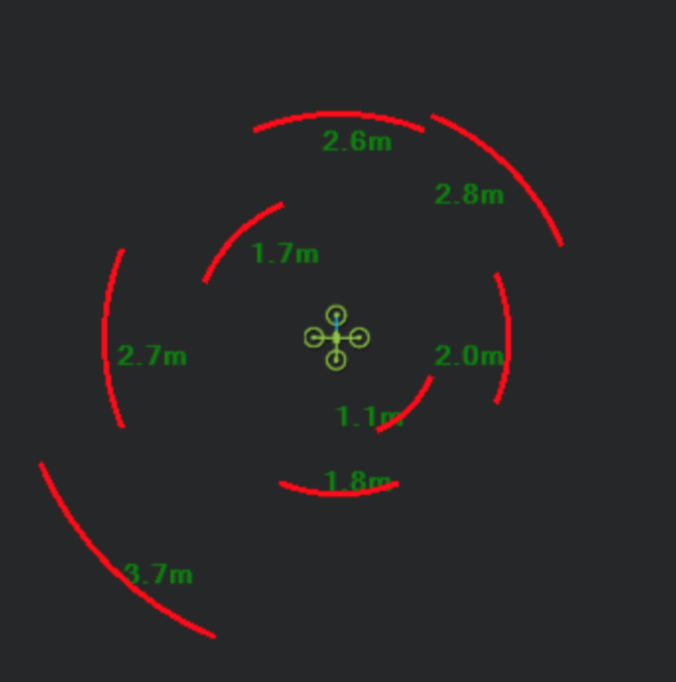
\includegraphics[width=0.3\linewidth]{./projects/logviewer/mission_planner_tower_evo.png}
    \caption{Data acquisition acknowledgement}
\end{figure}

\subsection{Sensors Integration and drone flight}
Drone integration
\begin{figure}[H]
    \centering
    \begin{subfigure}[b]{0.475\textwidth}
        \centering
        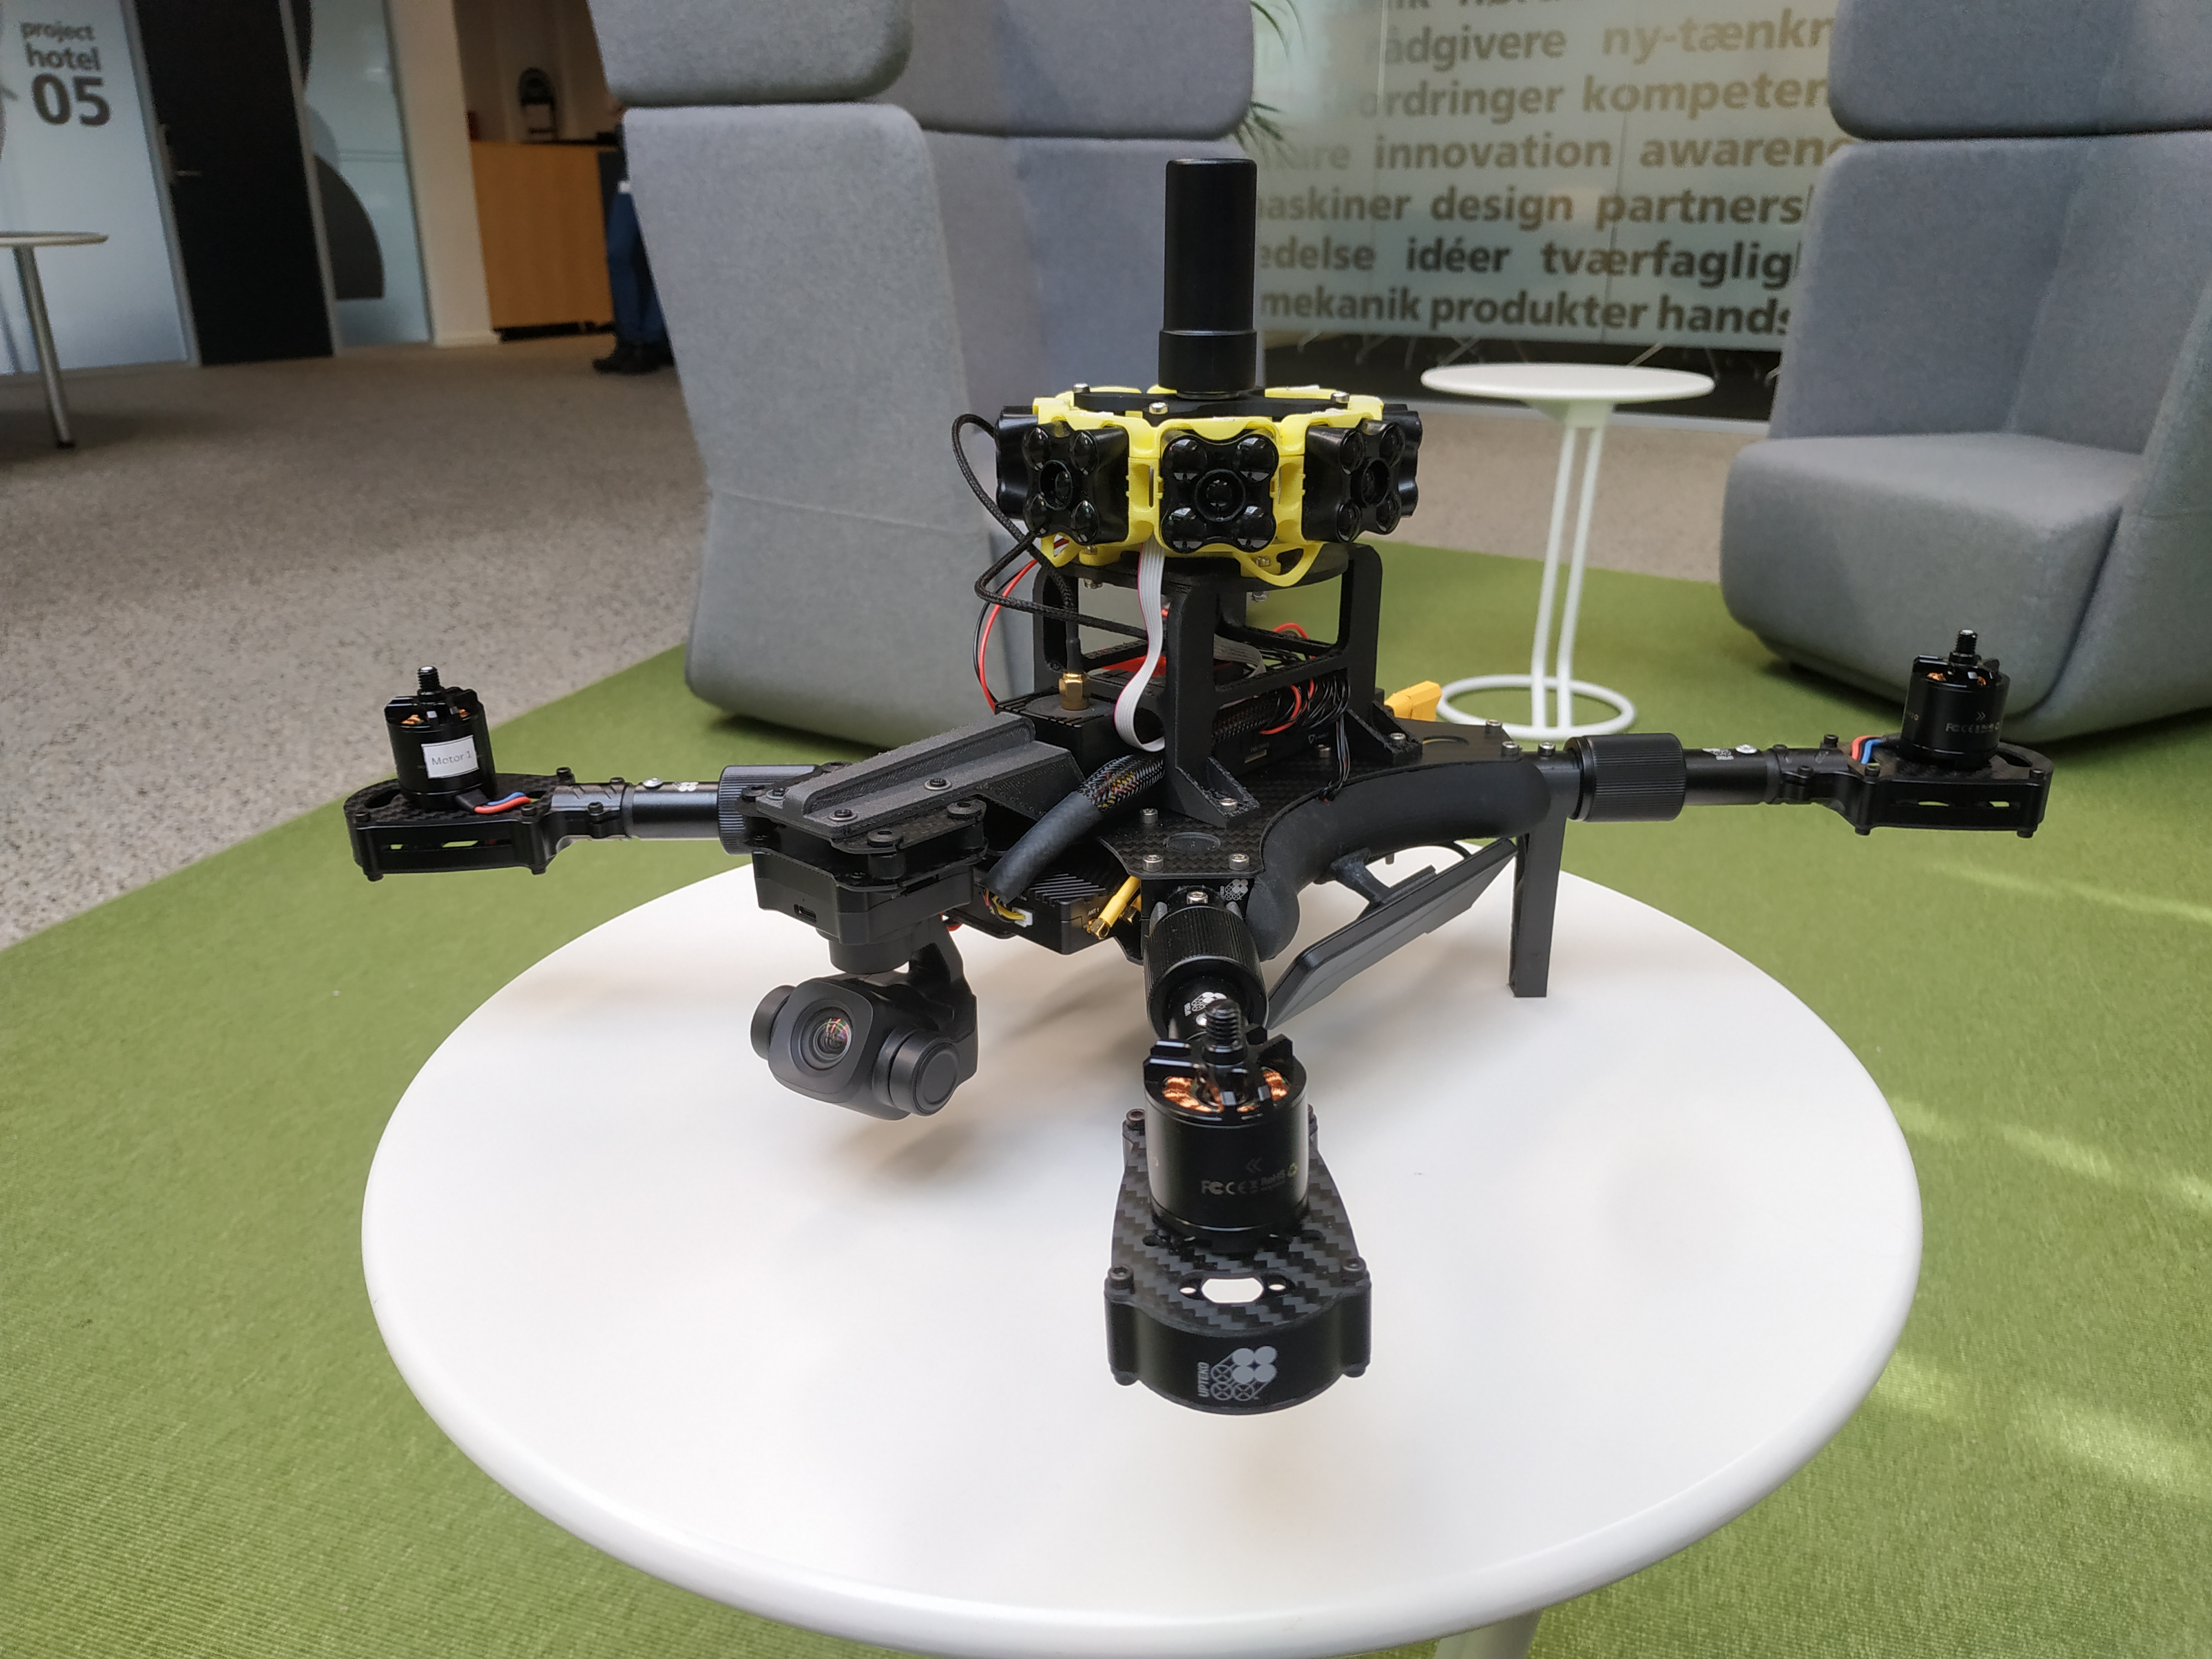
\includegraphics[width=\textwidth]{./projects/logviewer/drone_fl_view.jpg}
        \caption{Front left view}
    \end{subfigure}
    \hfill
    \begin{subfigure}[b]{0.475\textwidth}  
        \centering 
        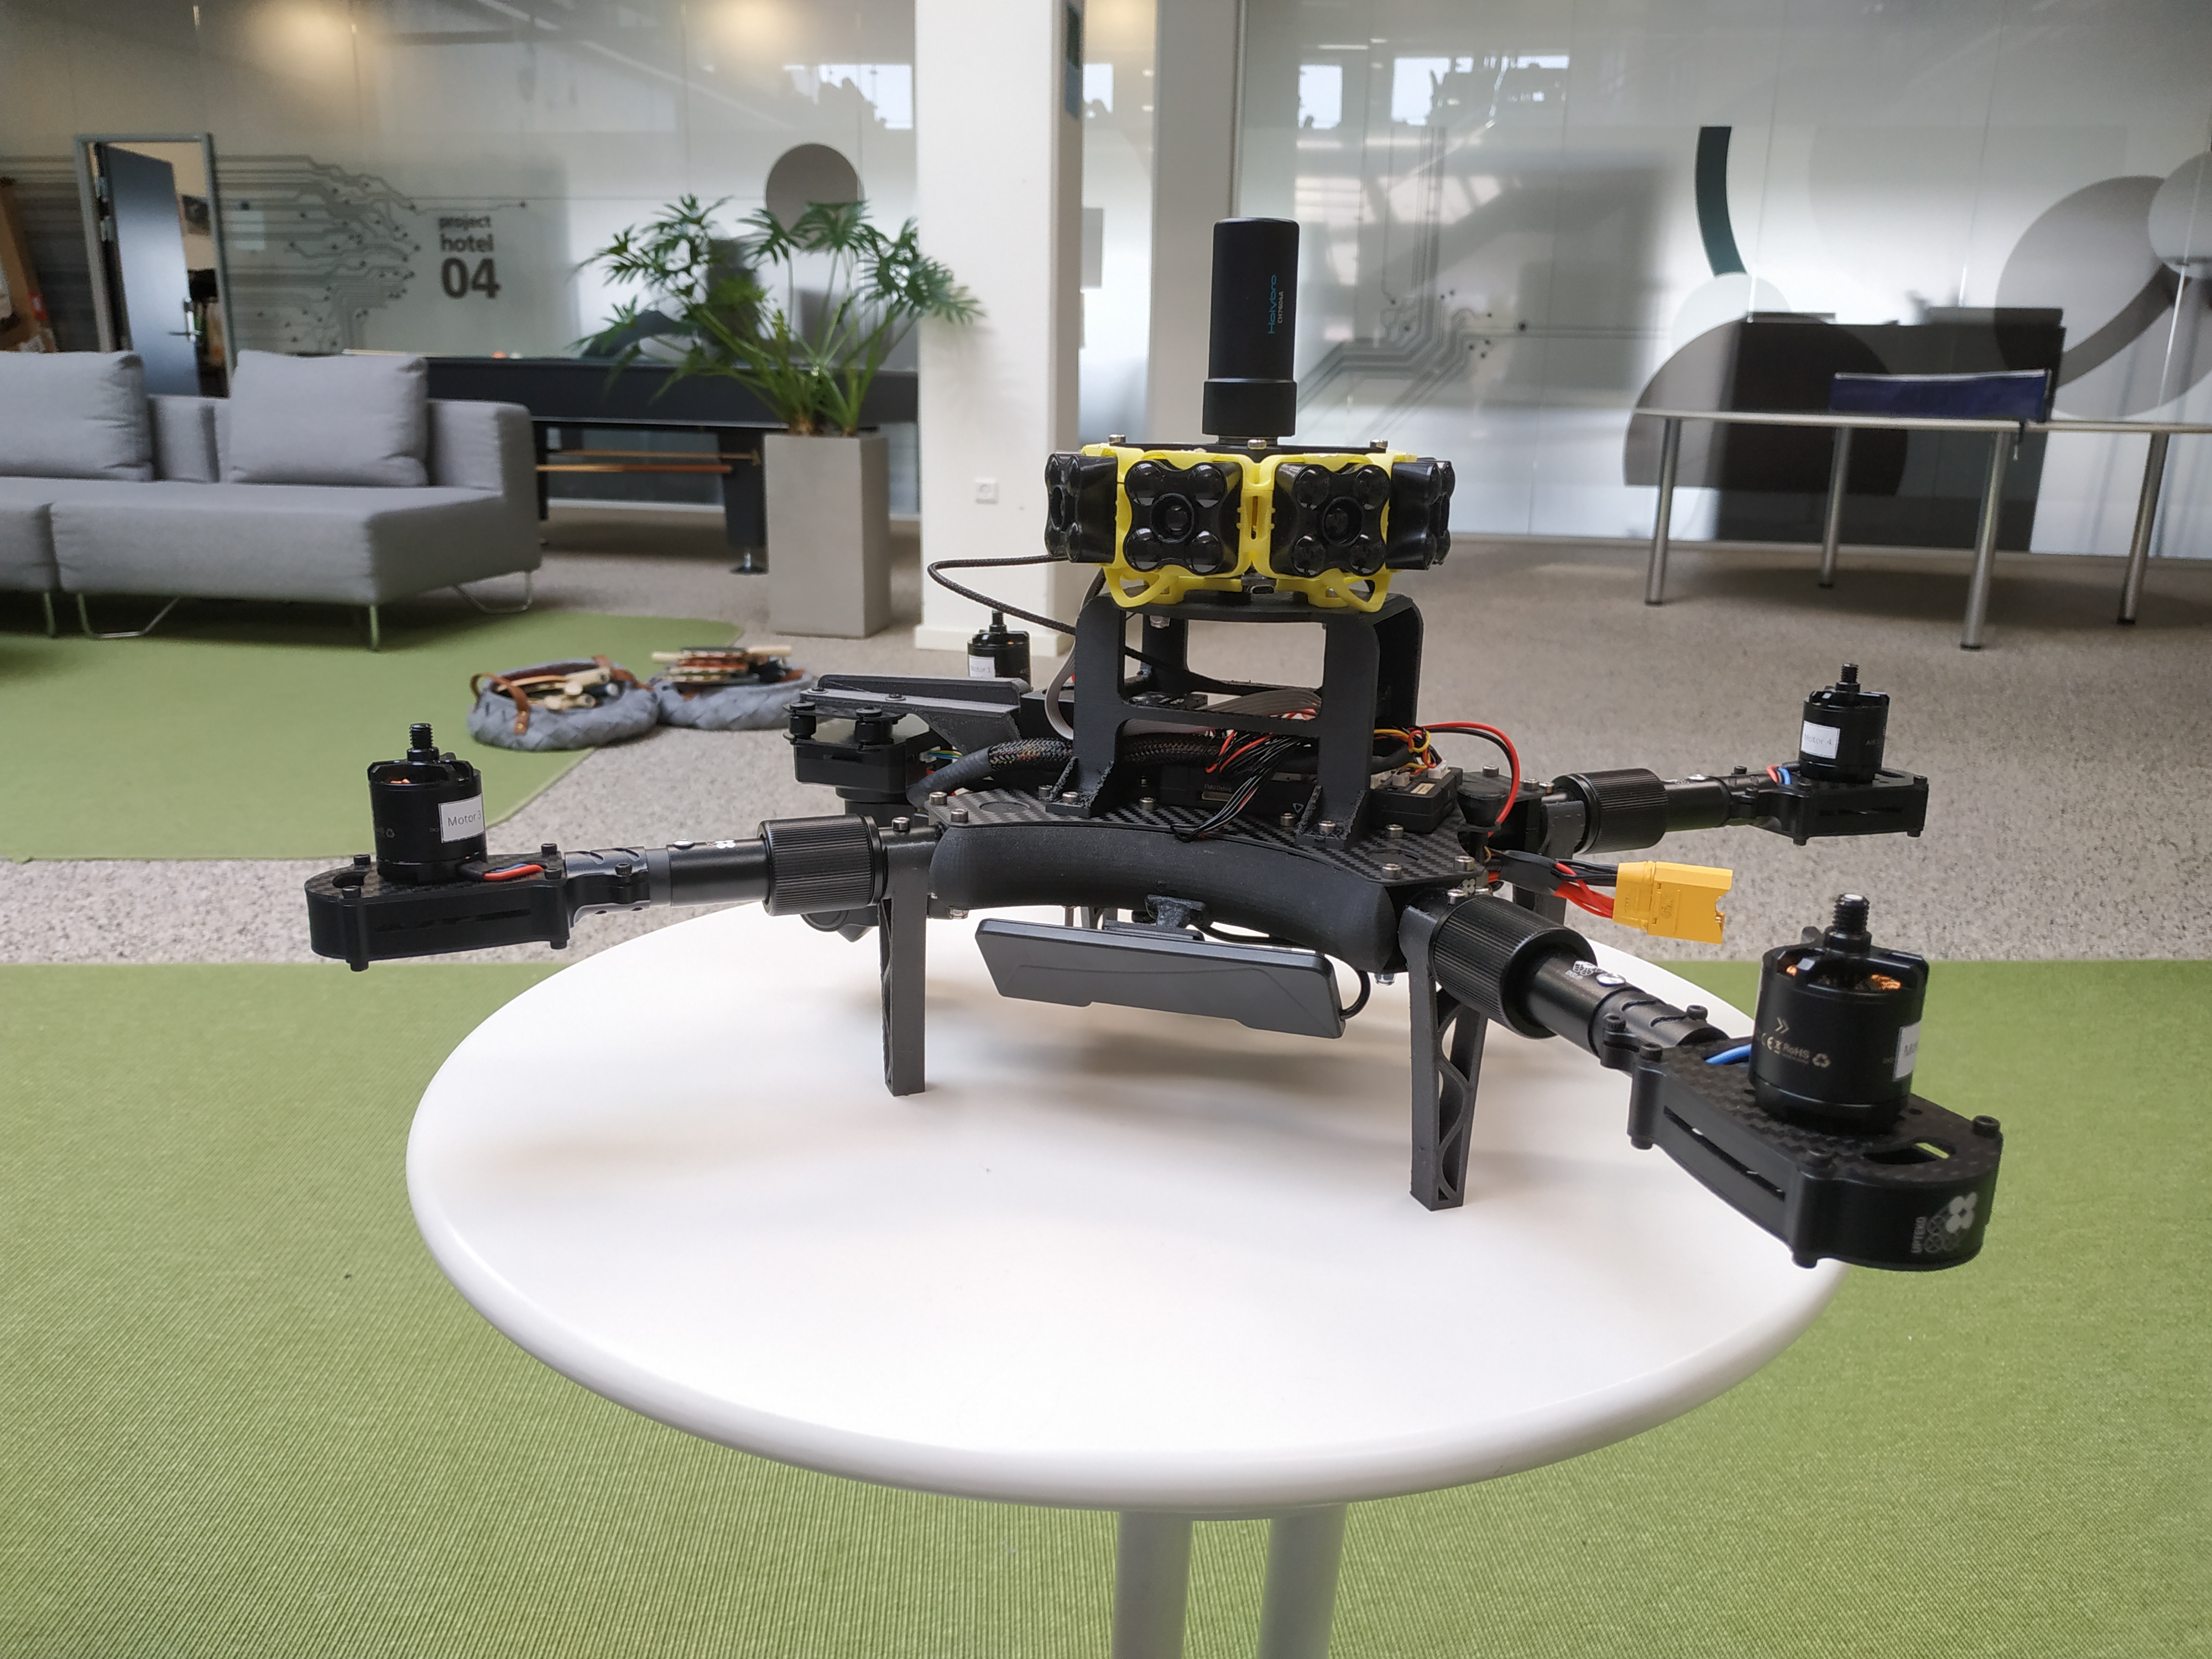
\includegraphics[width=\textwidth]{./projects/logviewer/drone_l_view.jpg}
        \caption{Left view}
    \end{subfigure}
    \vskip\baselineskip
    \begin{subfigure}[b]{0.475\textwidth}   
        \centering 
        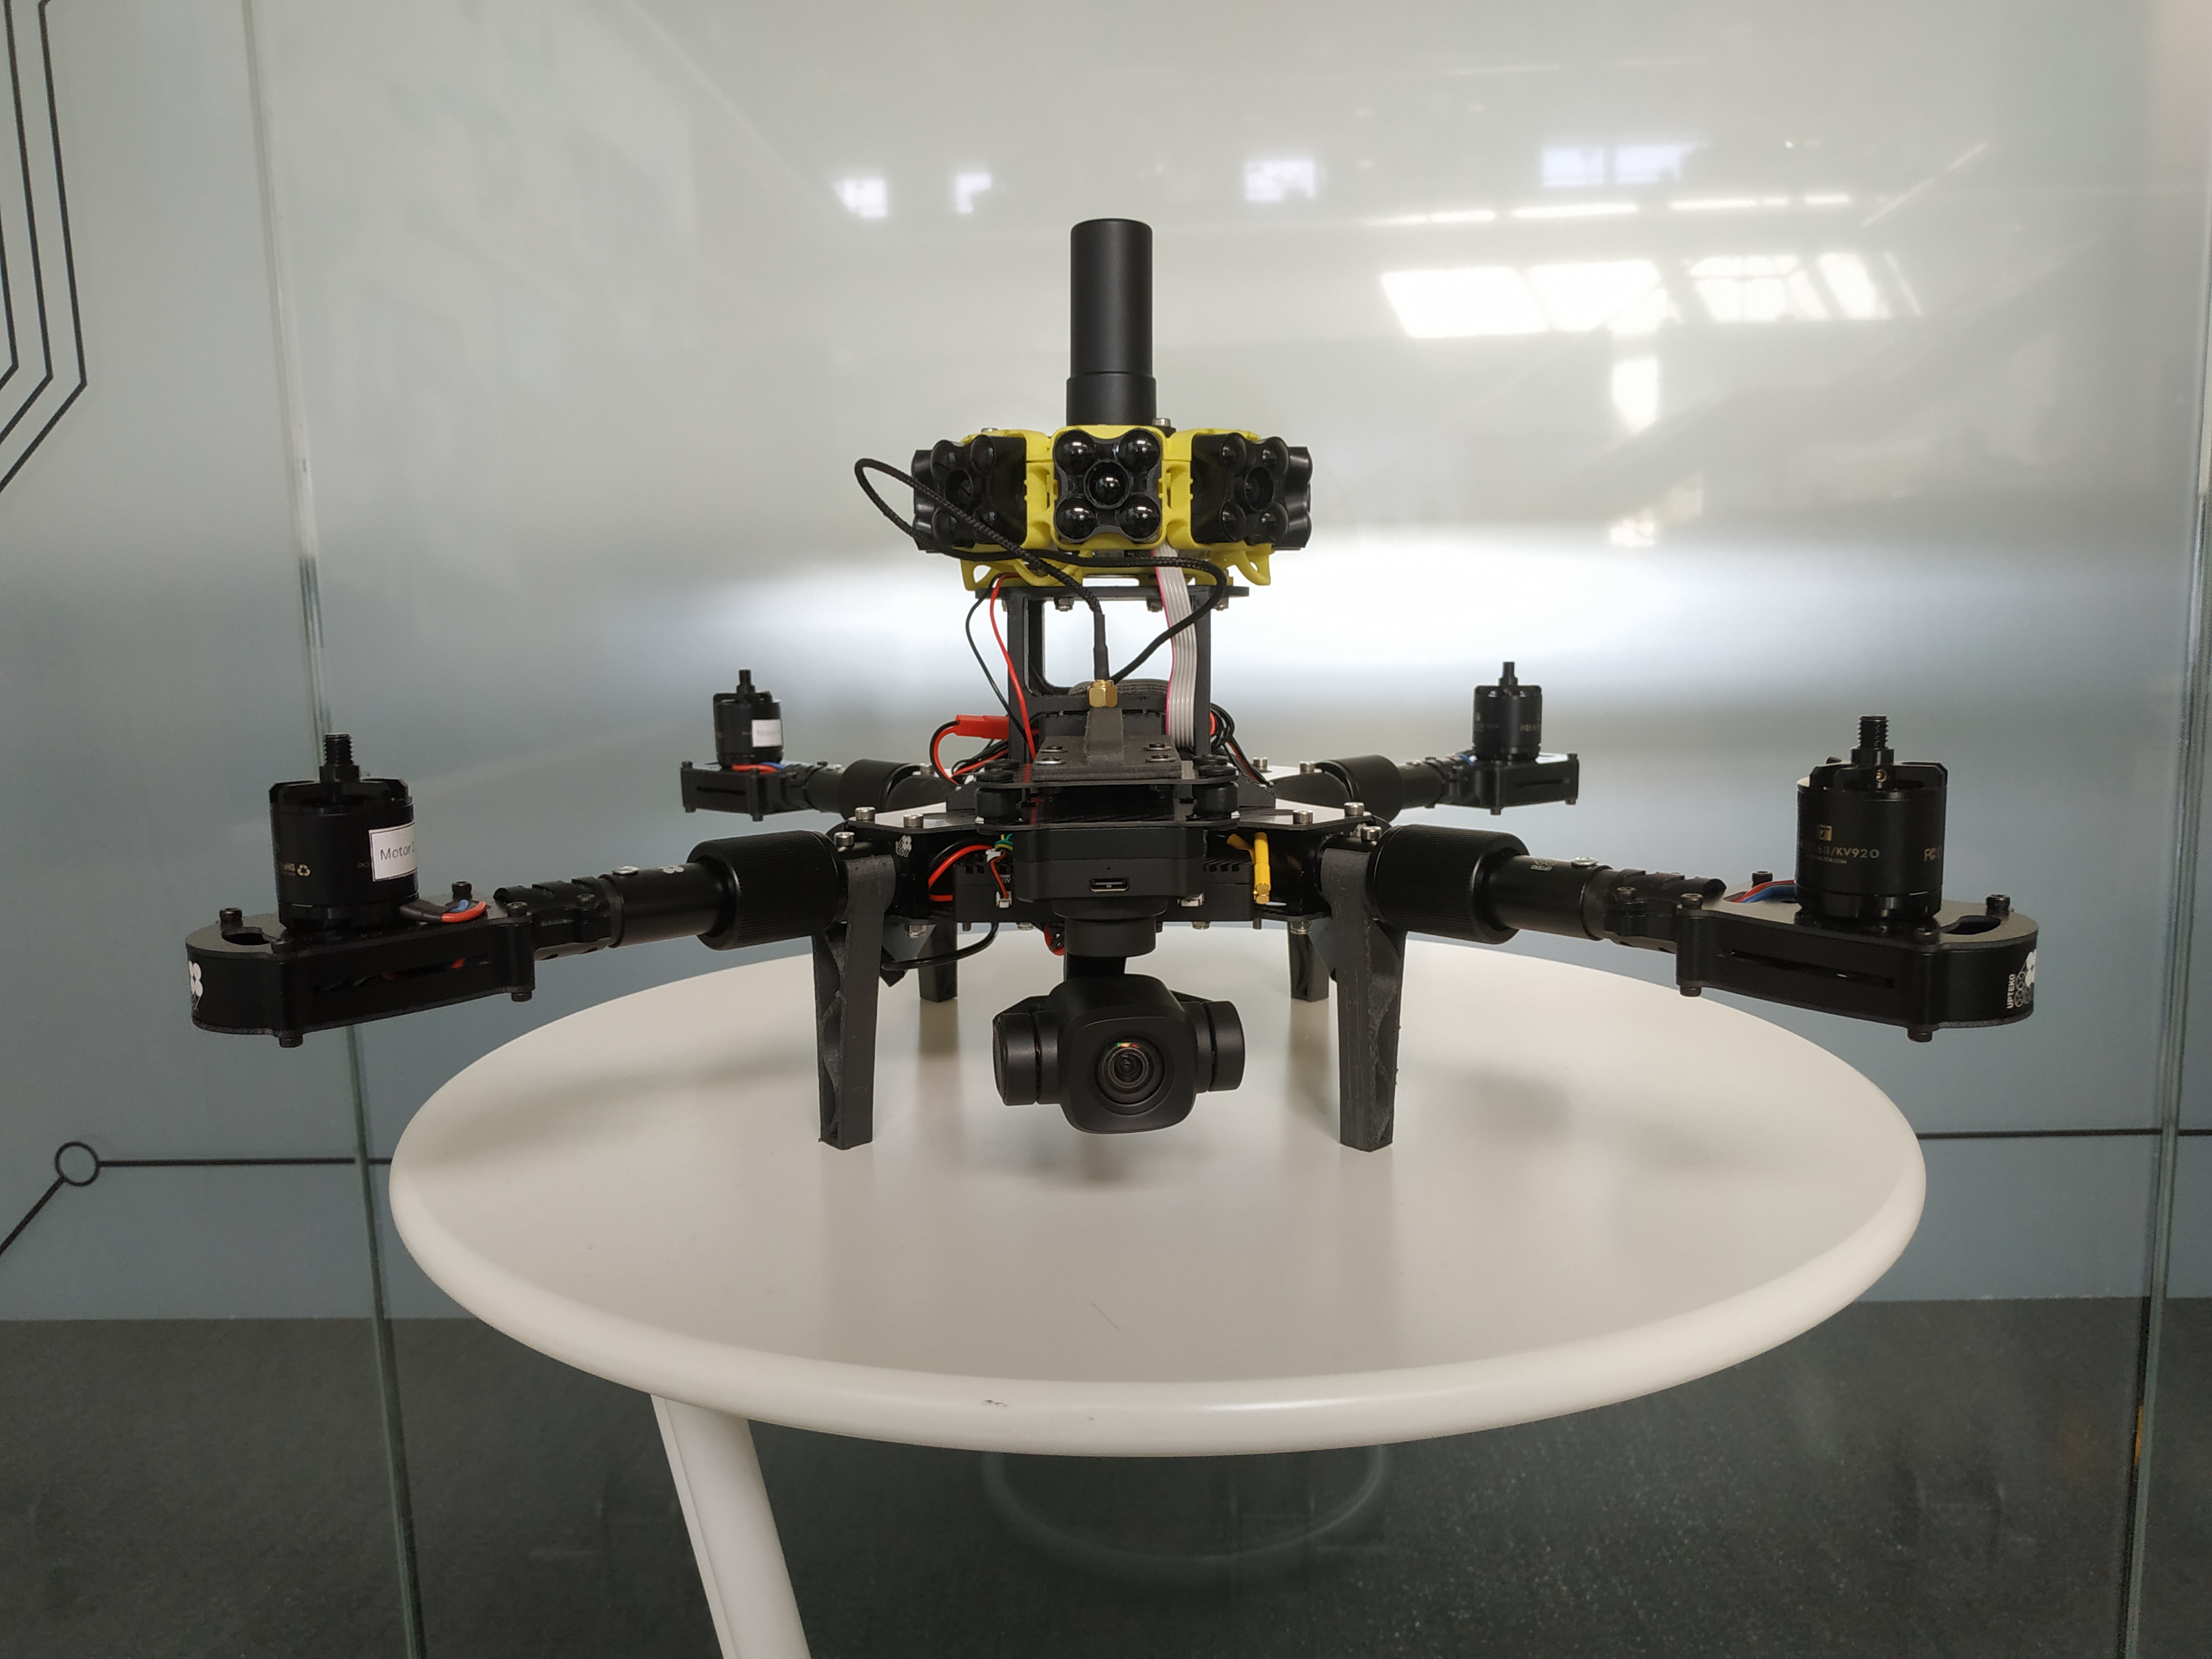
\includegraphics[width=\textwidth]{./projects/logviewer/drone_f_view.jpg}
        \caption{Front view}
    \end{subfigure}
    \hfill
    \begin{subfigure}[b]{0.475\textwidth}   
        \centering 
        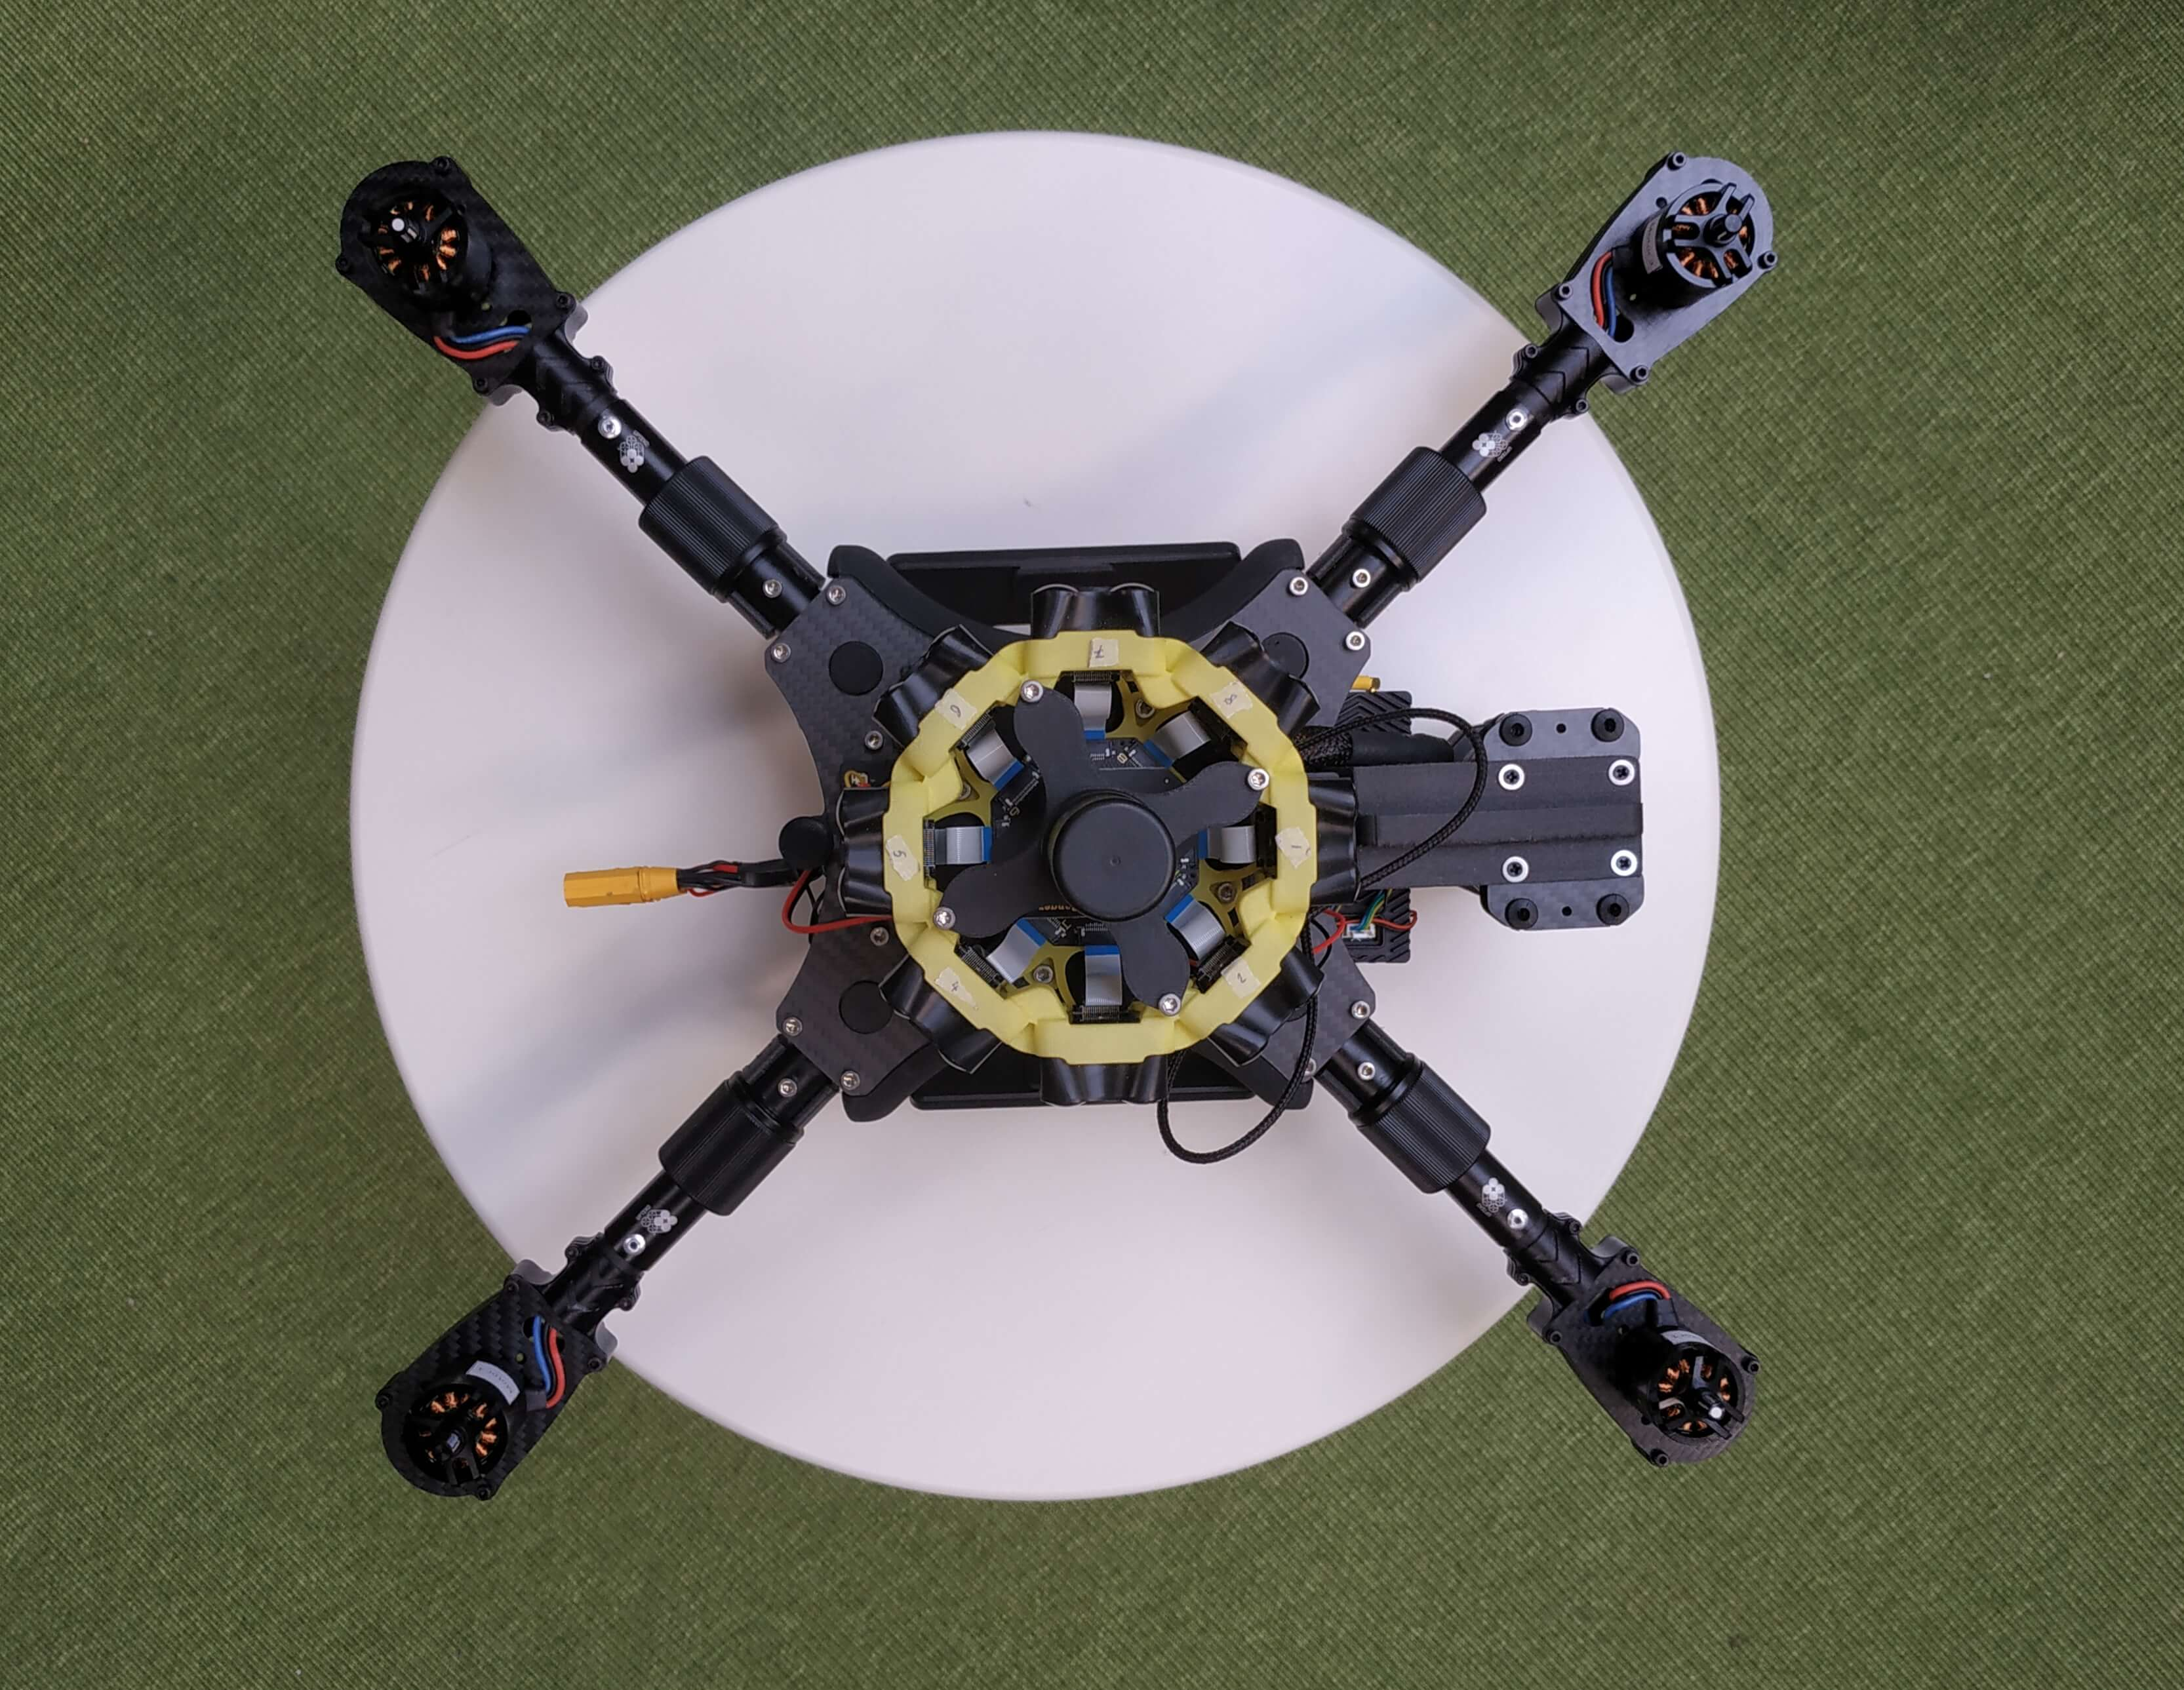
\includegraphics[width=\textwidth]{./projects/logviewer/drone_t_view.jpg}
        \caption{Top view}
    \end{subfigure}
    \caption{Larke Mini drone pictures with 360° degrees LIDAR mounted} 
\end{figure}


The drone successfully achieved its intended mission objectives. Whether it was aerial mapping and surveying, the drone effectively captured distance data.
My colleague Sebastian Duus ensured that the drone was in the optimal position for data acquisition, adjusting altitude and camera settings accordingly.

\subsection{Python Plotly Visualizer}
A graphical user interface is provided, leveraging \texttt{Plotly}\cite{plotly} library. The Logviewer import the \texttt{.csv} file as data.
Here is the \texttt{logfile.csv} header :
\begin{table}[H]
    \centering
    \begin{tabular}{|l|l|l|l|l|l|}
    \hline
    timestamp(ms) & PRX.D0 & PRX.D45 & PRX.D90 & PRX.D135 & PRX.D180 \\
    \hline
    PRX.D225 & PRX.D270 & PRX.D315 & ATT.Roll & ATT.Pitch & ATT.Yaw \\
    \hline
    \end{tabular}
    \caption{Plotly logviewer file header}
    \label{table:logfile_header}
\end{table}

The application is pretty simple : it use the timestamp as main variable to create animated data.
I created 3 main plots in th same window :
\begin{itemize}
    \item the distance sensors plot
    \item the roll and pitch attitude
    \item the yaw plot
\end{itemize}


The most valuable part of this application is the time slider that can be used to go back in time, pause and restart the view.
This way the data analysis is easy-to-use

\subsubsection{Final result}
% \begin{figure}[H]
%     \centering
%     \includegraphics{./projects/pmodnav/pmodnav_gui_record.gif}
%     \caption{Python GUI window GIF}
% \end{figure}

\section{Collision avoidance SITL}
\subsection{Environement description}
\subsubsection{Robot Operating System}
% ROS2 %
\texttt{ROS2} is an open-source framework for building robotic systems. It supports distributed systems, allowing communication between different components and nodes running on separate devices.
It provides a communication infrastructure for exchanging messages and supports various protocols. ROS 2 introduces a quality of service system for controlling communication behavior.
It includes real-time capabilities for time-critical applications. It supports multiple programming languages and emphasizes modularity and extensibility. ROS 2 comes with development tools and has an active community and ecosystem.
Overall, ROS 2 provides a powerful and versatile platform for developing robotic systems. Its distributed architecture, flexible communication infrastructure, real-time capabilities, language support, and extensibility make it a valuable tool for building complex and advanced robots.
\subsubsection{Gazebo}
% gazebo %
\texttt{Gazebo} is an open-source 3D simulation environment for robotics. It allows developers to create virtual worlds where they can simulate and test robots. Gazebo provides realistic physics-based simulations, visualizes the environment in 3D, and simulates sensors like cameras and lidars.
Users can model robots and their surroundings, integrate with the Robot Operating System (ROS), and extend its functionality using plugins. Gazebo has a supportive community and offers a wide range of resources for developers.
In summary, Gazebo is a valuable tool for simulating and evaluating robotic systems before deploying them in real-world environments.
\subsubsection{Ardupilot}
% ardupilot %
\texttt{Ardupilot} is open-source software used for controlling autonomous vehicles like drones. It includes firmware that runs on the vehicle's autopilot hardware, as well as ground control station software for mission planning and monitoring.
Ardupilot supports different flight modes, navigation based on waypoints, and telemetry for communication with the vehicle. It is compatible with various hardware platforms and can be customized and extended.
Ardupilot is widely used in drones and other vehicles, and it has a supportive community and extensive documentation. In summary, Ardupilot is a versatile and customizable software suite for autonomous vehicle control.

\subsection{Built-In Ardupilot collision avoidance}
The collision avoidance feature in Ardupilot is designed to enhance the safety and reliability of these vehicles by detecting and avoiding potential collisions with obstacles or other aircraft.

The collision avoidance system in Ardupilot relies on various sensors and algorithms to perceive the environment and make informed decisions about navigation. Some of the key components and techniques used in the Built-In Ardupilot collision avoidance include:

\begin{itemize}
    \item \underline{Sensor Inputs:} Ardupilot can interface with different types of sensors, including proximity sensors, lidar, sonar, and cameras. These sensors provide information about the surrounding environment and help in detecting obstacles.
    \item \underline{Obstacle Detection:} The collision avoidance system processes the sensor data to identify potential obstacles in the flight path. This can include buildings, trees, other aircraft, or any other objects that may pose a risk of collision.
    \item \underline{Path Planning:} Based on the environment map and the current position of the vehicle, Ardupilot generates a safe and collision-free path for the aircraft to follow. It considers factors such as obstacle proximity, vehicle speed, and maneuverability to calculate an optimal trajectory.
    \item \underline{Collision Avoidance Algorithms:} Ardupilot employs sophisticated algorithms to predict the future movement of obstacles and determine the best course of action to avoid collisions. These algorithms take into account the dynamics of the vehicle and the obstacles, allowing the autopilot to adjust the flight path accordingly.
\end{itemize}

% https://www.youtube.com/watch?v=W2ncr0DKWHE&ab_channel=IntelligentQuads

\begin{figure}[H]
    \centering
    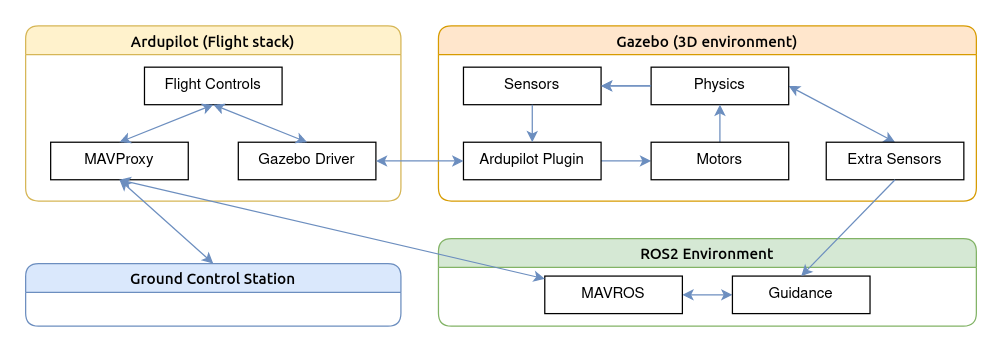
\includegraphics[width=0.65\linewidth]{./projects/ardupilot/sitl_overall.png}
    \caption{Software-In-The-Loop overall schematics}
\end{figure}

\subsection{Collision Avoidance ROS2 Migration}


\clearemptydoublepage
\backmatter
\chapter{Gantt Task Organization}
\begin{figure}[H]
    \centering
    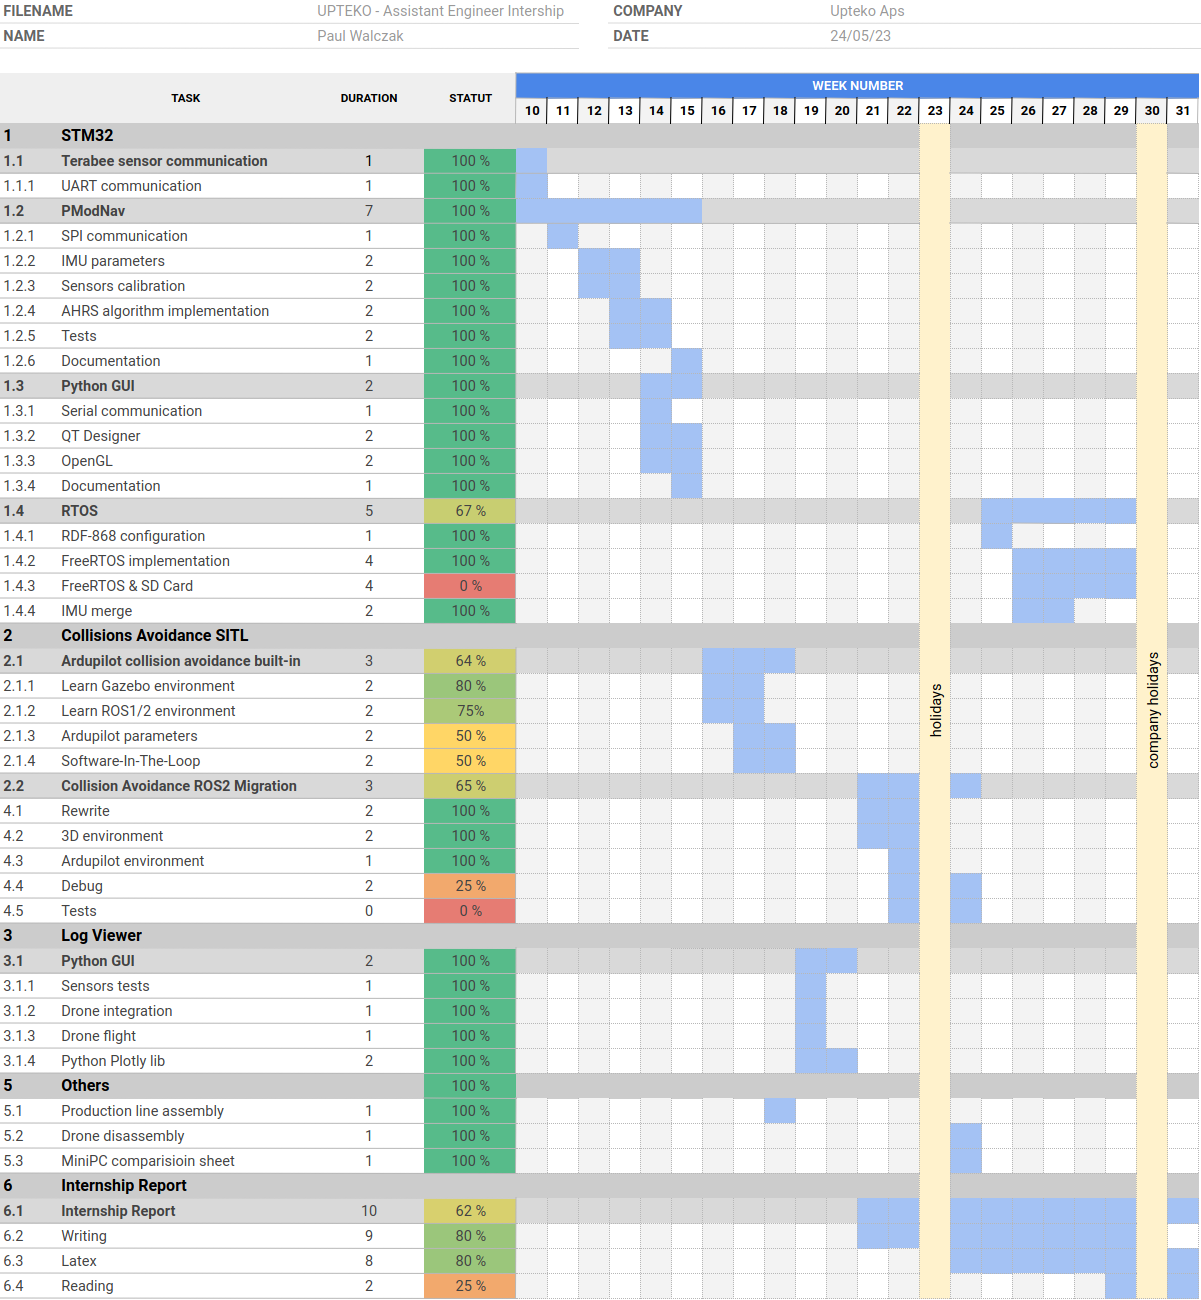
\includegraphics[width=0.94\linewidth]{./gantt/gantt.png}
    \caption{Gantt chart}
\end{figure}

\clearemptydoublepage
\backmatter
\chapter*{Conclusion}
\addcontentsline{toc}{chapter}{Conclusion}
\chaptermark{Conclusion}

%Upteko's rapid growth and constant stream of trainees does bring with it a few disadvantages. The most glaring one, in my opinion, is the fact that you can't "really" learn: \\
%In this type of company, the work environment is very varied, with hardware, software, simulation, fund-raising, professional events and so on. Each field has its own peculiarities and difficulties, and once you've discovered them, it's not all that easy to assimilate.
%I've been frustrated a few times when I've started to get used to a technology in order to be able to carry out a task in it, but have been unable to do so because of its complexity. It's a pity that I couldn't be helped or accompanied in these tasks, which are very interesting and quite unique.

The internship at Upteko was a unique and enriching experience that provided me with the opportunity to delve into various fields and technologies. The company's rapid growth and the constant influx of new trainees created a dynamic and stimulating work environment. However, this also presented certain challenges. The most significant of these was the difficulty in fully assimilating and mastering new technologies due to the breadth and complexity of the tasks at hand.
\\ \\
Despite the occasional frustrations, the experience was invaluable. It allowed me to apply the theoretical knowledge I had acquired in my academic studies to practical, real-world problems. The complexity of the tasks and the need for quick adaptation to new technologies and disciplines were significant learning experiences that will undoubtedly be beneficial in my future career.
\\ \\
However, I also recognized the need for more structured guidance and support in the learning process, particularly when dealing with complex technologies. This is an area where there is room for improvement in the company's internship program.
\\ \\
In conclusion, the internship was a journey of discovery and learning, offering a glimpse into the real-world applications of my academic knowledge. It provided me with a deeper understanding of the workings of a rapidly growing company and the challenges and opportunities that such an environment presents. Despite the challenges, I am grateful for the experience and the skills I have acquired, and I look forward to applying these in my future career.


% Chapitre pour la bibliographie
\clearemptydoublepage
\phantomsection % To have a correct link in the table of contents
\addcontentsline{toc}{chapter}{Bibliography}

% nocite: Pour citer la totalit\'{e} des r\'{e}f\'{e}rences contenues dans le fichier biblio
% nocite: In order to cite all the references included biblio
\nocite{*}
\printbibliography

\clearemptydoublepage
\printglossary[type=\acronymtype]

\clearemptydoublepage
\chapter*{Annexes}
\addcontentsline{toc}{chapter}{Annexes}

bla bla bla


\clearemptydoublepage
% Pour avoir la quatrième de couverture sur une page paire
% To have the back cover on an even page
\cleartoevenpage[\thispagestyle{empty}]

\markboth{}{}
% Plus petite marge du bas pour la quatrième de couverture
% Shorter bottom margin for the back cover
\newgeometry{inner=20mm,outer=20mm,top=40mm,bottom=20mm}

%insertion de l'image de fond du dos (resume)
%background image for resume (back)
\backcoverheader

% Switch font style to back cover style
\selectfontbackcover{ % Font style change is limited to this page using braces, just in case


\begin{multicols}{2}[\columnsep2em] 
    \smallTwelve{
    \noindent \textbf{Stagiaire}: Paul WALCZAK\\
    \noindent \textbf{Semestre}: Semestre 8\\
    \noindent \textbf{Entreprise}: Upteko ApS\\
    \noindent \textbf{Tuteur Entreprise}:Vincent KLYVERTS TOFTERUP\\
    \noindent \textbf{Tuteur ENIB}: Alexis MICHEL\\
    }
    \columnbreak
    \hfill
\includegraphics[keepaspectratio,height=3cm]{./cover/profile.png}
\end{multicols}


\subject{«Mon Sujet»} 

\keywords{«de 3 \`{a} 6 mots clefs»} 

\compagny{Eius populus ab incunabulis primis ad usque pueritiae tempus extremum, quod annis circumcluditur fere trecentis, circummurana pertulit bella, deinde aetatem ingressus adultam post multiplices bellorum aerumnas Alpes transcendit et fretum, in iuvenem erectus et virum ex omni plaga quam orbis ambit inmensus, reportavit laureas et triumphos, iamque vergens in senium et nomine solo aliquotiens vincens ad tranquilliora vitae discessit.
Hoc inmaturo interitu ipse quoque sui pertaesus excessit e vita aetatis nono anno atque vicensimo cum quadriennio imperasset. natus apud Tuscos in Massa Veternensi, patre Constantio Constantini fratre imperatoris, matreque Galla.
Thalassius vero ea tempestate praefectus praetorio praesens ipse quoque adrogantis ingenii.}

\resume{Eius populus ab incunabulis primis ad usque pueritiae tempus extremum, quod annis circumcluditur fere trecentis, circummurana pertulit bella, deinde aetatem ingressus adultam post multiplices bellorum aerumnas Alpes transcendit et fretum, in iuvenem erectus et virum ex omni plaga quam orbis ambit inmensus, reportavit laureas et triumphos, iamque vergens in senium et nomine solo aliquotiens vincens ad tranquilliora vitae discessit.
Hoc inmaturo interitu ipse quoque sui pertaesus excessit e vita aetatis nono anno atque vicensimo cum quadriennio imperasset. natus apud Tuscos in Massa Veternensi, patre Constantio Constantini fratre imperatoris, matreque Galla.
Thalassius vero ea tempestate praefectus praetorio praesens ipse quoque adrogantis ingenii, considerans incitationem eius ad multorum augeri discrimina, non maturitate vel consiliis mitigabat, ut aliquotiens celsae potestates iras principum molliverunt, sed adversando iurgandoque cum parum congrueret, eum ad rabiem potius evibrabat, Augustum actus eius exaggerando creberrime
docens, idque, incertum qua mente, ne lateret adfectans. quibus mox Caesar acrius efferatus, velut contumaciae quoddam vexillum altius erigens, sine respectu salutis alienae vel suae ad vertenda opposita instar rapidi fluminis irrevocabili impetu ferebatur.
Hae duae provinciae bello quondam piratico catervis mixtae praedonum.}

\conclusion{Eius populus ab incunabulis primis ad usque pueritiae tempus extremum, quod annis circumcluditur fere trecentis, circummurana pertulit bella, deinde aetatem ingressus adultam post multiplices bellorum aerumnas Alpes transcendit et fretum, in iuvenem erectus et virum ex omni plaga quam orbis ambit inmensus, reportavit laureas et triumphos, iamque vergens in senium et nomine solo aliquotiens vincens ad tranquilliora vitae discessit.
Hoc inmaturo interitu ipse quoque sui pertaesus excessit e vita aetatis nono anno atque vicensimo cum quadriennio imperasset. natus apud Tuscos in Massa Veternensi, patre Constantio Constantini fratre imperatoris, matreque Galla.}

\restoregeometry
}


\end{document}
